\chapter{各種の設定}

 TuneEditorは出力イメージ(jpegファイル)のレイアウトや文字/ドットの設定、キーボード割り当てなどを変更できるようになっています。

設定するための方法は、以下の3種類を用意しています。

\begin{quote}
\begin{description}
\item[URLパラメーターからの変更:] アプリ起動時のURLで設定を指定する方法です。URLパラメーターを指定した状態でブックマークとして登録しておけば、常にその設定で起動/使用できるようになります。
\item[メンテナンスダイアログボックスからの変更:] アプリケーション実行時にメンテナンス用のダイアログボックスから変更したい設定をひとつずつ指定する方法です。この設定はブラウザーのタブをクローズ/再ロードするまで有効となります。主な用途としては、実験的にパラメーターを変更して、その効果を確認するというものであり、次に説明する\texttt{.cfg}ファイルを作成する時に利用することができます。
\item[設定情報を書き込んだ\texttt{.cfg}ファイルからの変更:] ファイル入力ボタンから\texttt{.cfg}形式のファイルを読み込み、複数のパラメーターを一度に指定する方法です。この設定はブラウザーのタブをクローズ/再ロードするまで有効となります。
\end{description}
\end{quote}

設定できるパラメーターについては、\pageref{Parameters}ページを参照してください。

\textsf{注意点:}パラメーターのキーワードは大/小文字を意識しています。間違うと機能しないのでご注意ください。

\section{URLパラメーターからの変更}

 TuneEditorのURLの後ろには、「\textsf{キーワード}=\textsf{値}」という形式でパラメーターを記述していくことができるようになっています。この際、URLとパラメーターの間は「?」で区切り、複数のパラメーターを続けて指定するにはそれぞれのパラメーター間を「\&」で区切ってください。また、値に空白(`` '')が含まれる場合には、空白を「\texttt{\%20}」に変換してください。

\textsf{例}

\begin{verbatim}
https://〜省略〜/tuneEditor4.html?DotSSize=6&DotMSize=8&DotLSize=12
\end{verbatim}

※ この例は最小サイズのドット径を6、中サイズのドット径を8、最大サイズのドット径を12にするというものです。


\section{メンテナンスダイアログボックスからの変更}

 実行中に「\texttt{Ctrl+K}」キーを押下することで、\texttt{Enter override parameter (key=value format)}と表示されたメンテナンス用のダイアログボックスがオープンします。ここから指定したいパラメーターのキーワードと値を「=」で区切って入力します。


\section{設定情報を書き込んだ\texttt{.cfg}ファイルからの変更}

 テキストエディターを使用して、設定情報ファイルを作成します。設定ファイルの形式は、「\textsf{キーワード}=\textsf{値}」という指定を1行ずつ入力します。

\textsf{例}
\begin{quote}
\begin{verbatim}
DotSSize=6
DotMSize=8
DotLSize=12
\end{verbatim}
\end{quote}


\section{指定できるパラメーター}\label{Parameters}

\subsection{描画エリアの全体レイアウト}

 TuneEditorは出力イメージを作成するにあたり、最小の幅(\texttt{CanvasMinWidth})と最小の高さ(\texttt{CanvasMinHeight})という設定値から\textsf{最小限の描画領域}を作成し、その上下左右に余白(\texttt{CanvasTopMargin}, \texttt{CanvasBottomMargin}, \texttt{CanvasLeftMargin}, \texttt{CanvasRightMargin})を確保するようになっています。

なお、この最小限の描画領域の幅は、入力された行が長くなっていくと必要に応じて自動拡張されます。また、高さも改行が入力されるたびに、TSM行の高さ(\texttt{TSMHeight})と、行間表記を使う場合にはその高さ(\texttt{DotsAreaHeight})が加味されて自動的に拡張していくようになっています。

全体レイアウトに関するパラメーター群とデフォルト値は\pageref{GeneralParameters}ページにまとめてあります。


\subsection{TSM領域に関するパラメーター}

 TSM領域を管理するパラメーターには以下のものがあります。

\begin{quote}
\begin{description}
\item[\texttt{TSMHeight}] TSM領域の高さをピクセル単位で指定します。
\item[\texttt{TSMBaseLineOffset}] 該当行のTSM領域の最上部から見た文字のベースラインの位置をピクセル単位で指定します。
\item[\texttt{FontName}] フォント名称を指定します。
\item[\texttt{FontSize}] フォントサイズを指定します。なお、この使用は非推奨です(このパラメーターは通常の文字のサイズを指定するものであるため、TSM記号のサイズは変更されません--つまり使用すると文字とTSM記号のバランスが崩れてしまうのです)。
\end{description}
\end{quote}

TSM領域に関するパラメーター群とデフォルト値は\pageref{TSMParameters}ページにまとめてあります。

\subsection{行間表示領域に関するパラメーター}

 行間表示領域を管理するパラメーターには以下のものがあります。

\begin{quote}
\begin{description}
\item[\texttt{DotsSwitch}] 行間表示の使用有無を「0」か「1」で指定します。
\item[\texttt{DotsAreaHeight}] 行間表示領域の高さをピクセル単位で指定します。
\item[\texttt{TopLineOffset}] 該当行の行間表示領域の最上部から見た上限ラインの位置をピクセル単位で指定します。
\item[\texttt{BottomLineOffset}] 該当行の行間表示領域の最上部から見た上限ラインの位置をピクセル単位で指定します。
\item[\texttt{DotSSize}] 最小サイズのドット径をピクセル単位で指定します。
\item[\texttt{DotMSize}] 中サイズのドット径をピクセル単位で指定します。
\item[\texttt{DotLSize}] 最大サイズのドット径をピクセル単位で指定します。
\item[\texttt{GlideMagFactor}] 現在未使用。
\item[\texttt{DotDistributionPattern}] ドットの分布パターンを「0」〜「2」で指定します(後述)。
\item[\texttt{CentrelineSwitch}] センターラインの描画有無を「0」か「1」で指定します。
\end{description}
\end{quote}

ß
\begin{itembox}[l]{\textsf{ドットの配置パターンについて}}\label{dotdistribution}
上下線の間にサイズの異なるドットを縦方向に配分しようとした場合、いくつかのパターンが考えられます。

\medskip
\begin{itemize}
\item \textsf{設定「0」:}ドットの外周が上下線に接する位置を大/中/小のドットごとに計算し、中間の音は均等割りで配置する。
\medskip
\begin{center}
	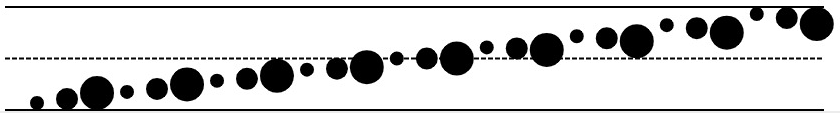
\includegraphics[width=10cm]{dd0.png}
 \end{center}
\medskip
\textsf{デメリット:}この場合、同じ高さの音でもドットのサイズが異なっている場合、中心の高さが異なって見える。
\medskip
\item \textsf{設定「1」:}最大のドットの外周が上下線に接する際のドットの中心位置を算出し、すべてのサイズのドットでその中心位置を使用するようにする。なお中間の音は均等割りで配置する。
\medskip
\begin{center}
	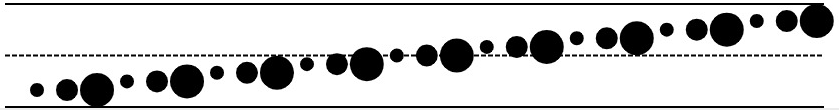
\includegraphics[width=10cm]{dd1.png}
 \end{center}
\medskip
\textsf{デメリット:}この場合、大サイズ以外のドットの外周は上下線に接することがなくなる。
\medskip
\item \textsf{設定「2」:}ドットの高さが最低/最高の場合にドットの外周が上下線に接するようにし、それ以外の場合には設定「1」を採用する。
\medskip
\begin{center}
	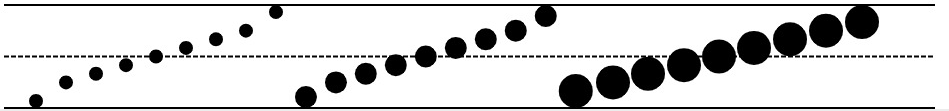
\includegraphics[width=10cm]{dd2.png}
 \end{center}
\medskip
\textsf{デメリット:}この場合、上昇調/下降調でドットを並べた場合、大サイズ以外のドットが直線上に並ばないケースが出てくる。
\end{itemize}

\medskip
なお、TuneEditorではこれら3つの戦略を起動時に選択することが可能になっています。

\end{itembox}


行間表示領域に関するパラメーター群とデフォルト値は\pageref{DotsAreaParameters}ページにまとめてあります。


\subsection{キーボード割り当て}

 各種のキーボード割り当ても変更することができますが、OSが規定しているキーボードショートカットと矛盾しないようなかたちで指定する必要があるため、思いがけない副作用に頭を抱えることになるかもしれません。

一般的な機能に対応付けられているキーボード割り当てパラメーター群とデフォルト値は\pageref{KeyboardParameters}ページにまとめてあります。

また、ドット操作に関するキーボード割り当てパラメーター群とデフォルト値は\pageref{DotOperationParameters}ページにまとめてあります。


\section{各種パラメーター(まとめ)}

\begin{table}[h]\label{GeneralParameters}
	\centering
	\caption{全体レイアウトに関するパラメーター}
	\smallskip
	\begin{tabular}{llr}
	\hline
	キーワード & 意味 & デフォルト値\\
	\hline
	\hline
	\texttt{CanvasMinWidth} & 最小限の描画領域の幅(ピクセル単位)
	 & 1000\\
	\hline
	\texttt{CanvasMinHeight} & 最小限の描画領域の高さ(ピクセル単位)
	 & 240\\
	\hline
	\texttt{CanvasTopMargin} & 全体画像の上部余白(ピクセル単位)
	 & 30\\
	\hline
	\texttt{CanvasBottomMargin} & 全体画像の上部余白(ピクセル単位)
	 & 30\\
	\hline
	\texttt{CanvasLeftMargin} & 全体画像の左余白(ピクセル単位)
	 & 30\\
	\hline
	\texttt{CanvasRightMargin} & 全体画像の右余白(ピクセル単位)
	 & 30\\
	\hline
	\end{tabular}
\end{table}

\begin{table}[h]\label{TSMParameters}
	\centering
	\caption{TSM領域に関するパラメーター}
	\smallskip
	\begin{tabular}{llr}
	\hline
	キーワード & 意味 & デフォルト値\\
	\hline
	\hline
	\texttt{TSMHeight} & TSM領域の高さ(ピクセル単位)
	 & 55\\
	\hline
	\texttt{TSMBaseLineOffset} & 文字のベースライン位置(ピクセル単位) & 40\\
	& (TSM領域の最上部からのオフセット) & \\
	\hline
	\texttt{FontName} & フォント名
	 & Times New Roman\\
	\hline
	\texttt{FontSize} & フォントサイズ(使用は非推奨)
	 & 27\\
	\hline
	\end{tabular}
\end{table}

\begin{table}[h]\label{DotsAreaParameters}
	\centering
	\caption{行間表示領域に関するパラメーター}
	\smallskip
	\begin{tabular}{llr}
	\hline
	キーワード & 意味 & デフォルト値\\
	\hline
	\hline
	\texttt{DotsSwitch} & 行間表示の有無(「0」は不要、「1」は要)
	 & 1\\
	\hline
	\texttt{DotsAreaHeight} & 行間表示の高さ & 130\\
	& (ピクセル単位) & \\
	\hline
	\texttt{TopLineOffset} & 行間表示開始位置と上限線のオフセット & 10\\
	& (ピクセル単位)& \\
	\hline
	\texttt{BottomLineOffset} & 行間表示開始位置と下限線のオフセット & 98\\
	& (ピクセル単位)& \\
	\hline
	\texttt{DotSSize} & 最小サイズのドット径(ピクセル単位)
	 & 5\\
	\hline
	\texttt{DotMSize} & 中サイズのドット径(ピクセル単位)
	 & 8\\
	\hline
	\texttt{DotLSize} & 最大サイズのドット径(ピクセル単位)
	 & 12\\
	\hline
	\texttt{GlideMagFactor} & 尻尾の倍率係数(実数)--現在未使用
	 & 1.00\\
	\hline
	\texttt{DotDistributionPattern} & ドット分布パターン  & 2\\
	\hline
	& (「0」〜「2」:\pageref{dotdistribution}ページを参照)  & \\
	\hline
	\texttt{CentrelineSwitch} & センターラインの有無 & 1\\
	& (「0」は不要、「1」は要) & \\
	\hline
	\end{tabular}
\end{table}

\begin{table}[h]\label{KeyboardParameters}
	\centering
	\caption{一般機能に関するキーボード割り当てパラメーター}
	\smallskip
	\begin{tabular}{llr}
	\hline
	キーワード & 意味 & デフォルト値\\
	\hline
	\hline
	\texttt{CursorLeft} & テキストカーソルを1文字分左に & ArrowLeft\\
	\hline
	\texttt{CursorRight} & テキストカーソルを1文字分右に & ArrorRight\\
	\hline
	\texttt{AnchorAndCursorLeft} & テキスト選択範囲を左に1文字分拡張 & Shift+ArrowLeft\\
	\hline
	\texttt{AnchorAndCursorRight} & テキスト選択範囲を右に1文字分拡張 & Shift+ArrowRight\\
	\hline
	\texttt{CursorUp} & テキストカーソルを1行上に & ArrowUp\\
	\hline
	\texttt{CursorDown} & テキストカーソルを1行下に & ArrowDown\\
	\hline
	\texttt{AnchorAndCursorUp} & テキスト選択範囲の1行上に拡張 & Shift+ArrowUp\\
	\hline
	\texttt{AnchorAndCursorDown} & テキスト選択範囲の1行下に拡張 & Shift+ArrowDown\\
	\hline
	\texttt{CursorHead} & テキストカーソルを行頭に & Ctrl+q\\
	\hline
	\texttt{CursorTail} & テキストカーソルを行末に & Shift+Ctrl+q\\
	\hline
	\texttt{CursorTail2} & テキストカーソルを行末に & Ctrl+w\\
	\hline
	\texttt{CursorTop} & テキストカーソルを文書頭に & Meta+ArrowUp\\
	\hline
	\texttt{CursorBottom} & テキストカーソルを文書末に & Meta+ArrowDown\\
	\hline
	\texttt{CursorPrevWord} & テキスト選択範囲を1ワード分前に & Shift+Ctrl+ArrowLeft\\
	\hline
	\texttt{CursorNextWord} & テキスト選択範囲を1ワード分後に & Shift+Ctrl+ArrowRight\\
	\hline
	\texttt{Backspace} & テキストカーソルの直前1文字を削除 & Backspace\\
	\hline
	\texttt{DeleteChar} & テキストカーソルの直後1文字を削除 & Delete\\
	\hline
	\texttt{CopyRegion} & 選択範囲をアプリ内の & Meta+c\\
	& バッファにコピー & \\
	\hline
	\texttt{CopyRegion2} & 選択範囲をアプリ内の & Ctrl+c\\
	& バッファにコピー & \\
	\hline
	\texttt{CutRegion} & 選択範囲をアプリ内の & Meta+x\\
	& バッファにコピーしカット & \\
	\hline
	\texttt{CutRegion2} & 選択範囲をアプリ内の & Ctrl+x\\
	& バッファにコピーしカット & \\
	\hline
	\texttt{Paste} & アプリ内のバッファからペースト & Meta+v\\
	\hline
	\texttt{Paste2} & アプリ内のバッファからペースト & Ctrl+v\\
	\hline
	\texttt{SelectAll} & テキスト全体を選択 & Meta+a\\
	\hline
	\texttt{SelectAll2} & テキスト全体を選択 & Ctrl+a\\
	\hline
	\texttt{MaintenanceHatch} & パラメーター設定ダイアログボックスの & Ctrl+k\\
	& オープン & \\
	\hline
	\end{tabular}
\end{table}

\begin{table}[h]\label{DotOperationParameters}
	\centering
	\caption{ドット操作に関するキーボード割り当てパラメーター}
	\smallskip
	\begin{tabular}{llr}
	\hline
	キーワード & 意味 & デフォルト値\\
	\hline
	\hline
	\texttt{StopAutoMove} & ドットの自動移動を抑止するキー & Shift\\
	\hline
	\texttt{WiderToneTail} & ドットの尻尾の幅を拡大する
	 & Shift+Meta+ArrowRight\\
	\hline
	\texttt{WiderToneTail2} & ドットの尻尾の幅を拡大する
	 & Ctrl+ArrowRight\\
	\hline
	\texttt{NarrowerToneTail} & ドットの尻尾の幅を縮小する
	 & Shift+Meta+ArrowLeft\\
	\hline
	\texttt{NarrowerToneTail2} & ドットの尻尾の幅を縮小する
	 & Ctrl+ArrowLeft\\
	\hline
	\texttt{RaiseToneTail} & ドットの尻尾の高さを拡大する
	 & Shift+Meta+ArrowUp\\
	\hline
	\texttt{RaiseToneTail2} & ドットの尻尾の高さを拡大する
	 & Ctrl+ArrowUp\\
	\hline
	\texttt{LowerToneTail} & ドットの尻尾の高さを縮小する
	 & Shift+Meta+ArrowDown\\
	\hline
	\texttt{LowerToneTail2} & ドットの尻尾の高さを縮小する
	 & Ctrl+ArrowDown\\
	\hline
	\texttt{RaiseToneTailEnd} & ドットの尻尾末尾の高さを上げる
	 & Shift+Ctrl+Meta+ArrowUp\\
	\hline
	\texttt{LowerToneTailEnd} & ドットの尻尾末尾の高さを下げる
	 & Shift+Ctrl+Meta+ArrowDown\\
	\hline
	\texttt{NextTone} & 次のドットにフォーカスを移す
	 & Shift+Meta+z\\
	\hline
	\texttt{NextTone2} & 次のドットにフォーカスを移す
	 & Shift+Ctrl+Z\\
	\hline
	\texttt{PrevTone} & 前のドットにフォーカスを移す
	 & Meta+z\\
	\hline
	\texttt{PrevTone2} & 前のドットにフォーカスを移す
	 & Shift+Ctrl+Z\\
	\hline
	\end{tabular}
\end{table}
